\noindent\textbf{1.} Phương trình chuyển động của viên bi:
\begin{equation*}
  m\vec{a}=-k\vec{r}+q\vec{v}\times\vec{B}
\end{equation*}
khi viên bi chuyển động trên quỹ đạo tròn bán kính $r_{0}$, gia tốc hướng tâm của nó có nguồn gốc từ lực từ và lực đàn hồi của sợi dây cao su, lực từ hướng vô trong hay hướng ra ngoài quỹ đạo phụ thuộc vào chiều chuyển động của hạt. Do đó, độ lớn vận tốc góc của hạt trong chuyển động này được xác định bởi:
\begin{equation*}
  m\omega^{2}r_{0}=kr_{0}=\pm qB\omega r_{0}\implies\omega^{2}\pm\frac{qb}{m}B-\frac{k}{m}=0
\end{equation*}
đặt $\Omega\equiv\dfrac{qB}{2m}$ và $\omega_{0}^{2}\equiv\dfrac{k}{m}$, độ lớn vận tốc góc của hạt khi nó chuyển động theo chiều kim đồng hồ là:
\begin{equation*}
  \omega_{1}=\sqrt{\omega_{0}^{2}+\Omega^{2}}+\Omega=\sqrt{\frac{k}{m}+\frac{q^{2}B^{2}}{4m^{2}}}+\frac{qB}{2m}
\end{equation*}
và khi chuyển động ngược chiều kim đồng hồ là:
\begin{equation*}
  \omega_{2}=\sqrt{\omega_{0}^{2}+\Omega^{2}}-\Omega=\sqrt{\frac{k}{m}+\frac{q^{2}B^{2}}{4m^{2}}}-\frac{qB}{2m}<\omega_{1}
\end{equation*}

\noindent\textbf{2.}
\begin{figure}[h]
  \centering
  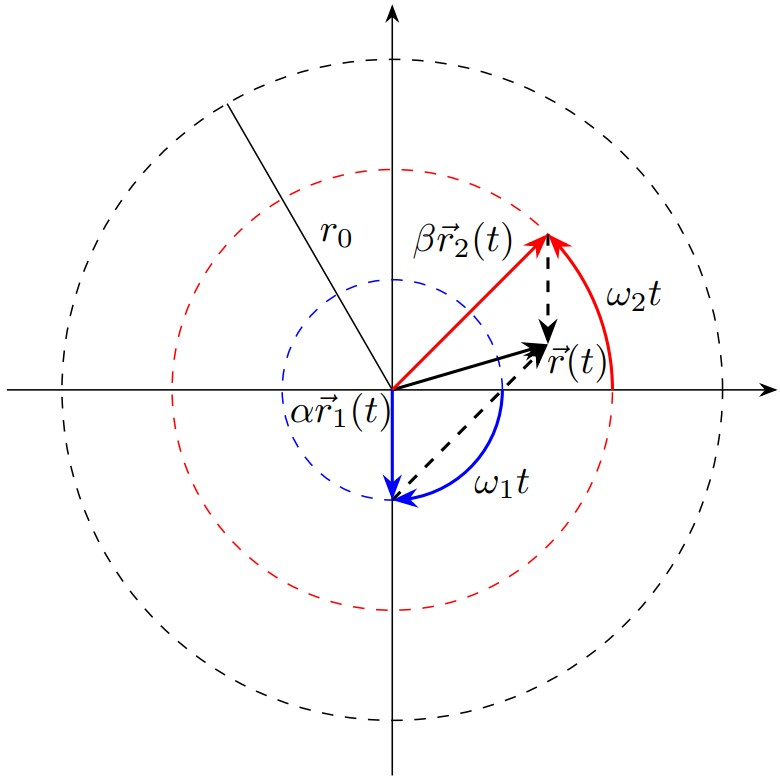
\includegraphics[width=0.55\textwidth]{Figures/Fig 1S1.jpg}
\end{figure}


\noindent Gọi $\vec{r}_{1}(t)$ và $\vec{r}_{2}(t)$ lần lượt là vector vị trí của viên bi khi nó chuyển động theo chiều kim đồng hồ và ngược chiều kim đồng hồ. Độ lớn vận tốc của viên bi trong mỗi trường hợp là $\lvert\vec{v}_{1}\rvert=\omega_{1}r_{0}$ và $\lvert\vec{v}_{2}\rvert=\omega_{2}r_{0}$ tương ứng. Nếu sự chồng chất của hai chuyển động này được biểu diễn dưới dạng:
\begin{equation*}
  \vec{r}(t)=\frac{\omega_{2}}{\omega_{1}+\omega_{2}}\vec{r}_{1}(t)+\frac{\omega_{1}}{\omega_{1}+\omega_{2}}\vec{r}_{2}(t)
\end{equation*}
thì theo tính đồng nhất của phương trình chuyển động, phương trình này cũng mô tả chính xác chuyển động mà chúng ta đang cần khảo sát. Thật vậy, ta có thể dễ dàng xác định các hệ số $\alpha$ và $\beta$ trong biểu thức của đề bài: vì $\vec{r}_{1}(0)=\vec{r}_{2}(0)\equiv\vec{r}_{0}$ và $\lvert\vec{v}_{1}(0)\rvert=\omega_{1}r_{0}=\dfrac{\omega_{1}}{\omega_{2}}\lvert\vec{v}_{2}(0)\rvert$ nên $\vec{r}(0)=0$ và $\vec{v}(0)=\vec{0}$. Như vậy, khoảng cách của viên bi tính từ lỗ khoan tại thời điểm $t$ là:
\begin{equation*}
  r^{2}(t)=\left(\frac{\omega_{2}}{\omega_{1}+\omega_{2}}r_{0}\right)^{2}+\left(\frac{\omega_{1}}{\omega_{1}+\omega_{2}}r_{0}\right)^{2}+2\frac{\omega_{2}}{\omega_{1}+\omega_{2}}r_{0}\cdot\frac{\omega_{1}}{\omega_{1}+\omega_{2}}r_{0}\cdot\cos[(\omega_{1}+\omega_{2})t]
\end{equation*}
suy ra:
\begin{equation*}
  r(t)=\frac{r_{0}}{\omega_{1}+\omega_{2}}\sqrt{\omega_{1}^{2}+\omega_{2}^{2}+2\omega_{1}\omega_{2}\cos[(\omega_{1}+\omega_{2})t]}
\end{equation*}
có thể thấy, tần số góc của viên bi trong chuyển động mới là $\omega_{1}+\omega_{2}=2\sqrt{\omega_{0}^{2}+\Omega^{2}}$, giá trị nhỏ nhất của $r(t)$ là:
\begin{equation*}
  r_{min}=\frac{\omega_{1}-\omega_{2}}{\omega_{1}+\omega_{2}}r_{0}=\frac{\Omega}{\sqrt{\omega_{0}^{2}+\Omega^{2}}}r_{0}
\end{equation*}

\noindent\textbf{3.} Từ phương trình của $r(t)$ có thể thấy rằng, khoảng cách lớn nhất của viên bi so với lỗ khoan là $r_{0}$, khoảng cách này đạt được tại những thời điểm:
\begin{equation*}
  t_{n}=\frac{\pi}{\sqrt{\omega_{0}^{2}+\Omega^{2}}}n\quad n=(0, 1, 2, \dots)
\end{equation*}
như vậy, thời gian từ lúc xuất phát đến khi $r(t)=r_{0}$ lần đầu tiên là:
\begin{equation*}
  \tau=\frac{\pi}{\sqrt{\omega_{0}^{2}+\Omega^{2}}}
\end{equation*}

\noindent\textbf{4.} Với tỷ lệ đã cho, ta có:
\begin{equation*}
  \vec{r}(t)=\frac{1}{3}\vec{r}_{1}(t)+\frac{2}{3}\vec{r}_{2}(t)
\end{equation*}
và:
\begin{equation*}
  r(t)=\frac{r_{0}}{3}\sqrt{5+4\cos(3\omega_{2}t)}
\end{equation*}
như vậy, chu kỳ chuyển động của viên bi là bội chung nhỏ nhất của chu kỳ của hai chuyển động thành phần, trong trường hợp này, chu kỳ chuyển động bằng với chu kỳ của chuyển động ứng với tần số góc $\omega_{2}$. Do đó, viên bi sẽ quay lại vị trí ban đầu sau:
\begin{equation*}
  T_{2}=\frac{2\pi}{\omega_{2}}=2\pi\sqrt{\frac{2m}{k}}
\end{equation*}
Chu kỳ thay đổi khoảng cách tới lỗ là:
\begin{equation*}
  T=\frac{2\pi}{\omega_{1}+\omega_{2}}=\frac{1}{3}T_{2}
\end{equation*}
cho nên trong một chu kỳ chuyển động, viên bi 3 lần đạt khoản cách lớn nhất $r_{0}$ và $3$ lần đạt khoảng cách nhỏ nhất $r_{0}/3$. Quỹ đạo hoàn chỉnh của viên bi sẽ $3$ lần đi qua đường tròn lớn bán kính $r_{0}$ và $3$ lần đi qua đường tròn nhỏ bán kính $r_{0}/3$; ở các điểm tiếp xúc với đường tròn lớn, viên bi sẽ di chuyển theo phương bán kính, trong khi đó, ở các điểm tiếp xúc với đường tròn nhỏ, viên bi sẽ di chuyển theo phương tiếp tuyến với đường tròn. Dựa vào các thông tin trên, ta có thể vẽ được quỹ đạo của hạt:
\begin{figure}
  \centering
  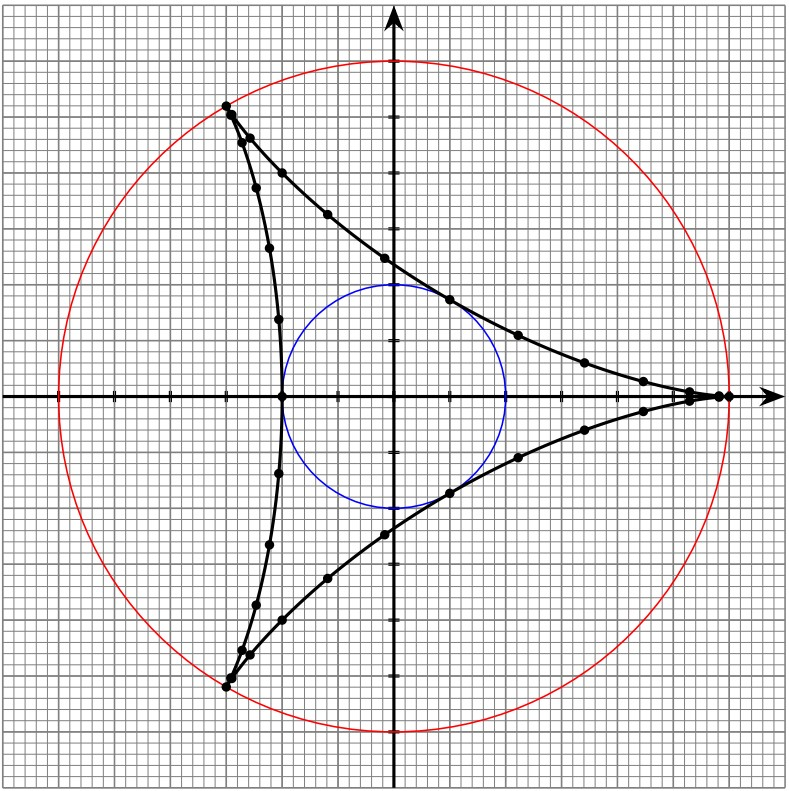
\includegraphics[width=0.65\textwidth]{Figures/Fig 1S2.jpg}
\end{figure}
